%!TEX root = /Users/zolkko/Projects/zolkko-alarm/doc/main.tex
\section{Реализация программно-аппаратного комплекса <<Универсальная система
терморегулирования на базе микроконтроллера AVR семейства XMega>>}
В качестве объекта исследования в ходе выполнения дипломного проектирования мной
была спроектирован и частично реализован программно-аппаратный комплекс
универсального терморегулирования.

Одной из возможных областей применения такого рода комплексов является дистанционное
автоматизированное управление коптильными камерами, используемыми при изготовлении
колбасных изделий фабрик пищевой промышленности.

\subsection{Описание структурной схемы универсальной системы терморегулирования}
Структурная схема универсальной системы терморегулирования на базе микроконтроллера
AVR семейства XMega приведена в приложении A.

По функциональному назначению разрабатываемый программно-аппаратный комплекс условно
разделён на три больших функциональных блока.

\begin{par}
	1.	Управляющее устройство -- устройство устанавливаемое непосредственно
	на объект управления. Выполняет следующие функции:
		\begin{itemize}
			\item{} ОУ -- чтение показаний термопар и усиление их сигнала;
			\item{} устройство индикации -- выводит информацию о текущем состоянии системы;
			\item{} память -- хранит настройки системы и список технологических процессов для
				исполнения;
			\item{} звуковая сигнализация -- выполняет оповещение звуковым сигналом о
				наступлении события завершения текущей операции или о том, что произошла ошибка;
			\item{} устройство ввода -- обеспечивает функцию задания операции на исполнение,
				остановку операции исполнения;
			\item{} датчик температуры -- получение температур холодного спая термопары;
			\item{} блок ШИМ управления -- формирует управляющий сигнал, воздействующий на
				тепло-электро нагреватель;
			\item{} сетевой интерфейс -- обеспечивает функцию передачи и приёма данных
				через сеть Ethernet 802.3;
			\item{} центральный процессов -- модуль обеспечивающий взаимодействие компонентов
				управляющего устройства, направленное на исполнение заданного технологического
				процесса.
		\end{itemize}
\end{par}

\begin{par}
	2.	Контролирующий сервис -- обеспечивает:
	 	\begin{itemize}
			\item{} авторизацию устройства управления;
			\item{} сбор и хранение показаний датчиков управляющего устройства;
			\item{} интерфейс пользователя контролирующей системы.
		\end{itemize}
\end{par}

\begin{par}
	3.	Объект управления -- объект, управление и контроль состояния которого необходимо проводить
		в данном технологическом процессе.
\end{par}



\subsection{Детализация компонентов универсальной системы терморегулирования}
При реализации было использовано несколько компонентов.

\begin{par}
	1.	Центральный микроконтроллер -- микроконтроллер atxmega128a3. Микропрограмма контролера
	составлена таким образом, что прерывание модуля RTC происходит с частотой 100 Гц.
	При приходе прерывания микроконтроллер отсчитывает количество $ \frac{1}{100} $ с. прошедших с момента
	включения схемы и выполняет запрос на обновление состояния всех дочерних объектов.
	Программа микроконтроллера написана на языке C++ для компилятора входящего в поставку
	AVR-GCC 4.3.3.
\end{par}
	
\begin{par}
	2.	В качестве устройства индикации используется TFT ЖК-дисплей DST\-2001\-PH \cite{display} со встроенным
	драйвером ili9320 включённым в режиме system i80 16-бит\cite{ili9320}.
	Так как количество портов ввода\--вывода на используемом микроконтроллере достаточно, введение дополнительных узлов
	расширяющих возможности ввода\--вывода микроконтроллера -- не предусмотрено.
	\begin{figure}[ht]
		\center{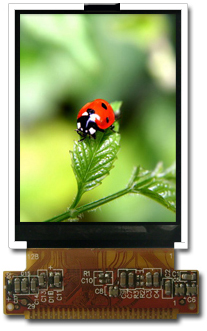
\includegraphics[bb=0 0 150 250, clip, scale=0.5]{ili9320.png}}
		\caption{Внешний вид TFT ЖК-дисплея DST2001PH}
		\label{img:iili9320}
	\end{figure}
\end{par}

\begin{par}
	3.	Модуль ввода данных пользователя выполнен на сенсорном экране ЖК-дисплея,
	выполненного по 4-проводной схеме включения резистивного сенсорного экрана. Для
	оцифровки значений получаемых с сенсорного экрана должны использоваться АЦП\cite{avradc} центрального
	микроконтроллера.
\end{par}
	
\begin{par}
	4.	Звуковое оповещение о наступившем событии выполнено на широко распространённой
	микросхеме mc34119, включённой в стандартном режиме (рис. \ref{img:mc34119m}).
	\begin{figure}[ht]
		\center{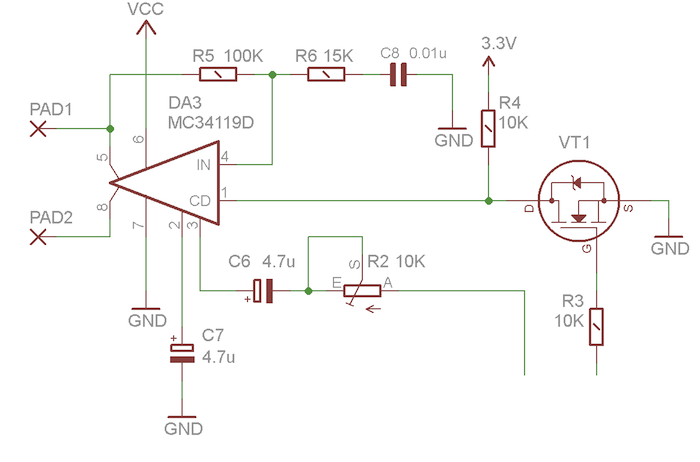
\includegraphics[bb=0 0 700 480, clip, scale=0.5]{mc34119.png}}
		\caption{Схема включения mc34119}
		\label{img:mc34119m}
	\end{figure}
	Управление сигналом Chip Disable микросхемы производиться ключом на транзисторе VT1. Низкий уровень
	переводит микросхему в состояние низкого энергопотребления \cite{mc34119}.
	
	Для надёжного перехода микросхемы усилителя необходимо производить выдержку не менее 40 мс.
	Сигнал на УНЧ подаётся с цифро-аналогового преобразователя микроконтроллера.
\end{par}

\begin{par}
 	5.	В качестве памяти устройства используется энергонезависимые карты памяти MicroSD.
	Применение этого вида памяти позволяет не прибегая к перепрограммированию устройства
	вносить конфигурационные данные в систему. В случае недоступности внешней памяти микроконтроллер использует
	встроенную память EEPROM.
\end{par}

\begin{par}
 	6.	В качестве контролера сетевого интерфейса используется микросхема фирмы Micro Chip
	enc28j60. Пример включения этого микроконтроллера дан на рисунке \ref{img:ienc28j60}.
	\begin{figure}[ht]
		\center{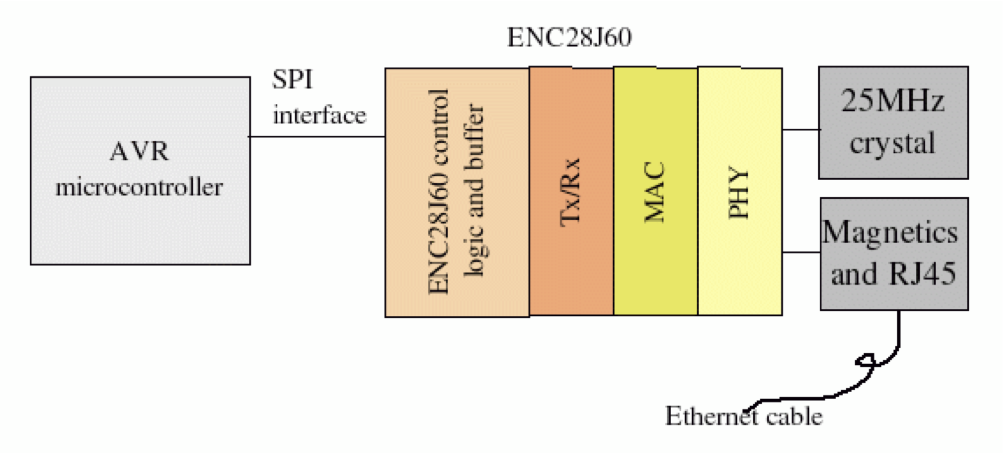
\includegraphics[bb=0 0 500 220, clip, scale=0.6]{enc28j60.png}}
		\caption{Схема включения микроконтроллера enc28j60}
		\label{img:ienc28j60}
	\end{figure}
	
	Этот микроконтроллер требует использования трансформатора с отношением 1:1 сертифицированного
	для сетей 10base-T. По этому для упрощения изделия необходимо использовать готовые RJ45
	коннекторы ''Magjack'', которые включают в своей конструкции необходимые трансформаторы и
	свето диоды. В случае использования этого метода в схему устройства необходимо будет добавить
	только одну индуктивность в 10 мкГн.
	
	Взаимодействие центрального микроконтроллера и микросхемы сетевого интерфейса осуществляется
	по протоколу SPI \cite{enc28j60}, расширенному дополнительными сигнальными линиями. Методика
	использования модуля SPI приведена в официальной документации \cite{avrspi}.
\end{par}


\subsection{Анализ динамики работы системы}
В процессе разработки любой системы крайне важным шагом является проведение анализа динамики
работы разрабатываемой системы.
В качестве инструмента анализа динамики программных систем часто используются диаграммы последовательности (рисунок \ref{img:dynamic}),
так как они являются удобным средством для обозначения очерёдности следования сообщений от одного объекта к другому во времени.
\begin{figure}[ht]
	\center{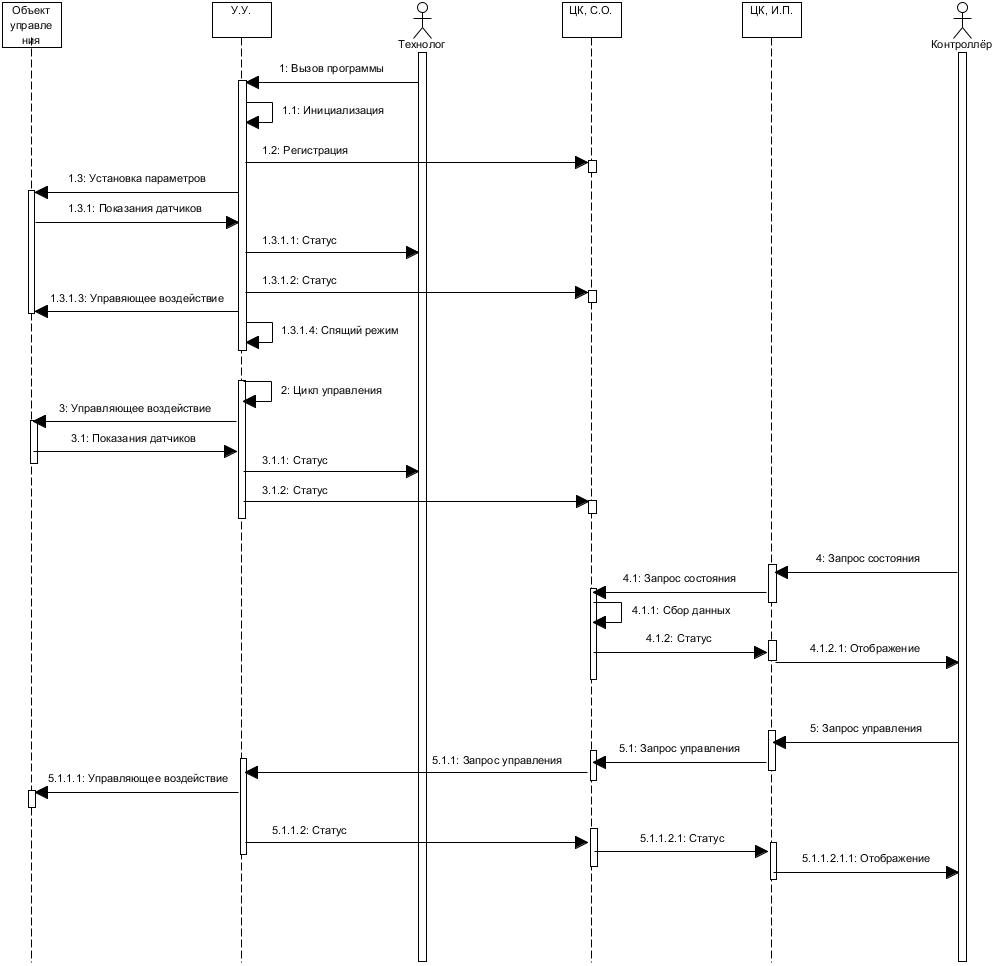
\includegraphics[bb=0 0 250 250, clip, scale=1.8]{system_dynamic.png}}
	\caption{Диаграмма динамики системы}
	\label{img:dynamic}
\end{figure}
Главный акцент диаграммы последовательности -- порядок и динамика поведения, то есть как и в каком порядке происходят события.

\subsection{Разработка контролирующего сервиса}
Из представленной диаграммы динамики работы системы (рисунок \ref{img:dynamic}), видно,
что контролирующий сервис выполняет обработку исключительно коротких запросов. Однако, количество таких
запросов довольно большое.

Применение сервисов выделяющих на обработку каждого запроса отдельного потока может привести к
ситуации, когда политика операционной системы заблокирует выделение дополнительного потока сервису,
или постоянное переключение между выполняющимися равнозначными потоками приводит к значительным задержкам
в обработке одного запроса, из-за больших накладных расходов на переключение контекстов операционной системы.

В случае использования сервисов с выделенным ограниченным пулом потоков возможно возникновение ситуации, когда
из-за большого наплыва запросов, используемый пул потоков исчерпывается и сервис вынужден ставить вновь
пришедший запрос в очередь, что так же сказывается на скорости реакции системы.

Одним из возможных способов решения обозначенных проблем является применение <<лёгких>> потоков и написание кода
обработчиков сетевых запросов таким образом, что бы не возникала необходимость производить их синхронизацию.


Наиболее простым и эффективным способом добиться этого -- является применение специализированных библиотек или
систем программирования. Язык программирования ErLang изначально проектировался для решения проблем
многопоточности. А разработанная в его рамках и технология OTP, не только обеспечивает хорошую структурируемость
системы, но и позволяет производить горизонтальное масштабирование всей системы за счёт распределения нагрузки
между несколькими узлами.

Структура разработанного контролирующего сервиса представлена на рисунке \ref{img:otpStruct}.
\begin{figure}[ht]
	\center{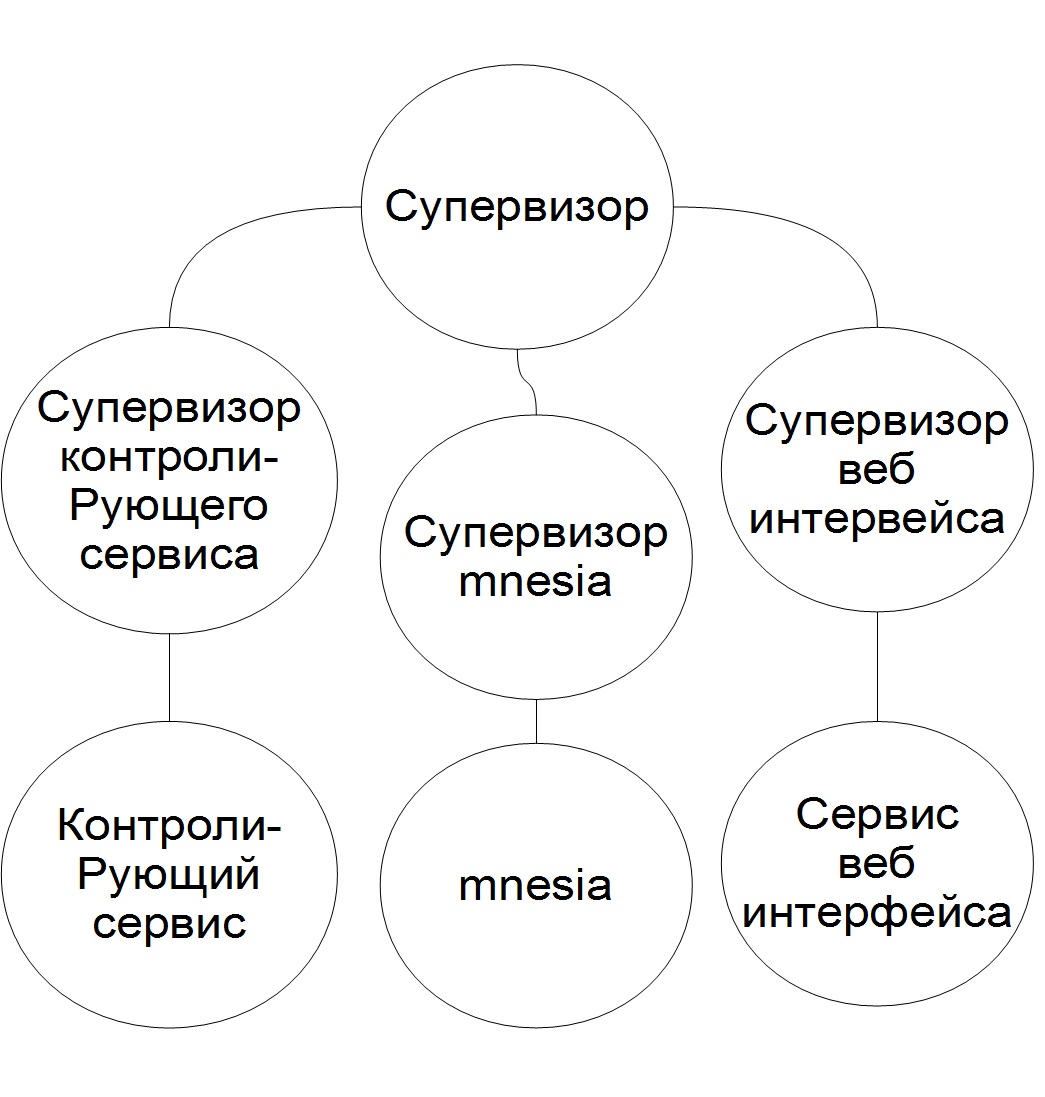
\includegraphics[bb=0 0 850 800, clip, scale=0.4]{otp_struct.png}}
	\caption{Дерево контроля контролирующего сервиса}
	\label{img:otpStruct}
\end{figure}

Система состоит из трёх рабочих процессов:
\begin{enumerate}
	\item конролирующий сервис -- обеспечивающий взаимодействие с устройствами управления;
	\item сервис базы данных -- приложение распределённой докумен-ориентированной базы данных,
	хранящей журнал выполненных операций, список опрашиваемых узлов и прочие параметры,
	необходимые для функционирования системы;
	\item веб-сервис -- серверное приложение предоставляющее интерфейс пользователя (оператора)
	к функциям.
\end{enumerate}

Каждый из рабочих процессов контролируется своим собственным супервизором, каждый из которых управляется
корневым супервизором.


\subsubsection{Методика обеспечения отказоустойчивости контролирующего сервиса}
Основной концепцией в Erlang/OTP является дерево контроля. Это модель структурирования процессов,
основанная на идее рабочих и контролеров \cite{otpOv}. Её составными частями являются:

\begin{itemize}
	\item рабочие -- это процессы, которые выполняют вычисления, и, собственно, выполняют основную работу;
	\item супервизоры -- это процессы, которые контролируют поведение рабочих;
	\item дерево контроля -- это иерархическое разделение кода на контролеров и рабочих,
		позволяющее разрабатывать устойчивое к ошибкам программное обеспечение.
\end{itemize}

В случае возникновения ошибки в программном обеспечении написанном в соответствии с приведённой структурой,
супервизор произведёт перезапуск рабочего процесса. Политика реакции на ошибки определяется во время регистрации
рабочих процессов в супервизоре при его создании.

Ещё одним плюсом использования такой архитектуры сервисов является возможность распределения
сетевых служб по зонам безопасности. То есть контролирующий сервис и приложение базы данных можно разворачивать
в безопасной сетевой зоне, доступ в которую есть только у внутренних ресурсов. Веб-сервис же можно разворачивать
в демилитаризованной зоне, не опасаясь, что злоумышленник причинит вред приложению.

Не маловажным является и возможность осуществления двойного контроля выполняемых действий. На первом шаге
веб-сервис выполняет проверку правильности ввода пользователя, на втором -- контролирующий сервис
может произвести проверку адекватности выполняемых функций.


\subsection{Разработка сервиса обслуживания запросов операторов системы}
В целях обеспечения надёжности функционирования контролирующего сервиса, что обеспечивается его
 изоляцией в локальной сети предприятия, функции предоставления интерфейса пользователя оператора
и обслуживания запросов операторов были реализованы в дополнительном веб-сервисе.

В отличии от контролирующего сервиса, необходимости ограничивать доступ к веб-сервису из внешних
сетей отсутствует, так как он не позволяет осуществлять ни каких деструктивных функций
операторам системы. Его взаимодействие с базой данных состояния системы осуществляется только по чтению,
а все запросы на управляющие устройства проводятся исключительно через контролирующий сервис.

Как и контролирующий сервис, веб-сервис написан на языке программирования ErLang с использованием технологий
OTP. Подход при котором в качестве веб-сервиса используется частная реализация службы, а не готовый веб-сервис
общего назначения, позволяет повысить производительность системы, уменьшить время её отклика, за счёт реализации
только минимально необходимой для функционирования логики.

Применение архитектуры OTP при разработке веб-сервиса так же позволяет в случае необходимости горизонтальной
распределить нагрузку.

Горизонтальное масштабирование веб-сервиса можно произвести следующими способами:
\begin{itemize}
	\item создание нескольких веб-сервисов на разных сетевых интерфейсах работающих с одним экземпляром
		контролирующего сервиса;
	\item создание одного веб-сервиса, но нескольких узлов с логикой обратного вызова веб-сервиса;
	\item создание нескольких узлов веб-сервисов, каждый из которых обслуживает свой собственный узел
		контролирующего сервиса.
\end{itemize}


Веб интерфейс оператора (рисунок \ref{img:acsIf}) контролирующего сервиса позволяет использовать в качестве
ПЭВМ контролирующего сервиса практически любой современный компьютер, в том числе планшетные компьютеры, нет-топы.
За счёт этого, возможно сократить количество дополнительного оборудования, необходимого для обслуживания и использования
системы при её внедрении.

\begin{figure}[ht]
	\center{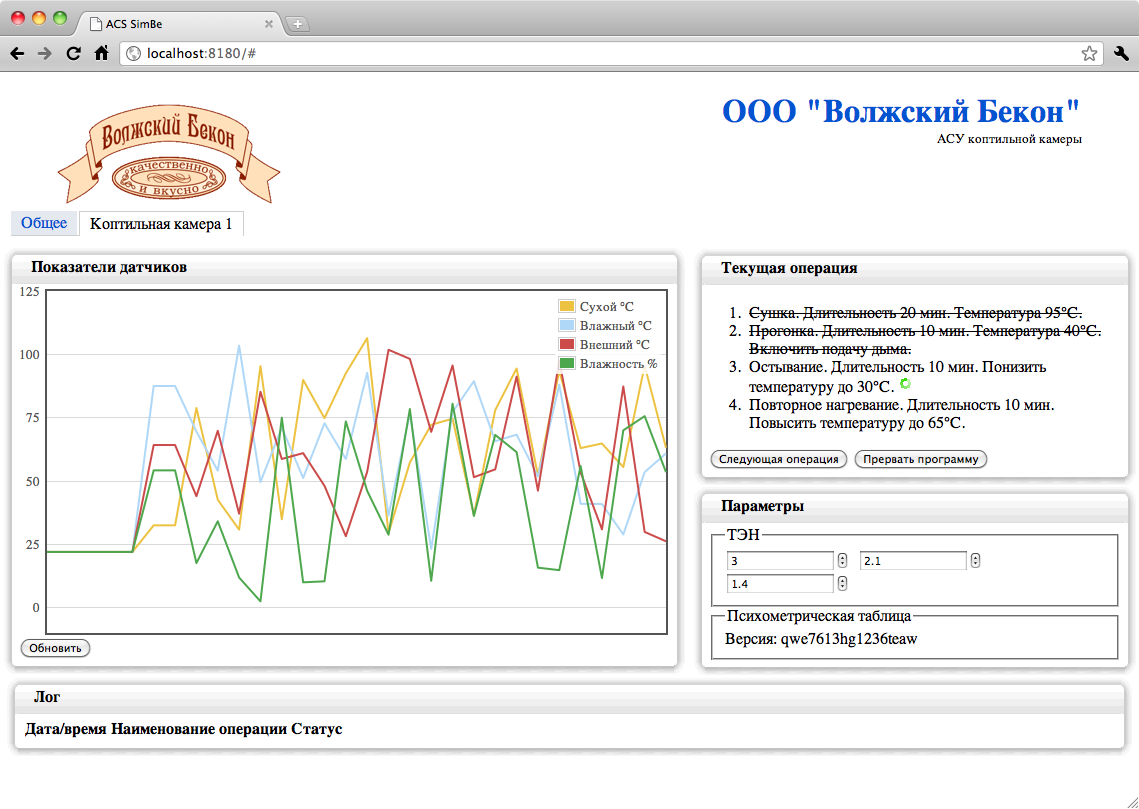
\includegraphics[bb=0 0 1200 800, clip, scale=0.4]{acs_if.png}}
	\caption{Интерфейс оператора контролирующего сервиса}
	\label{img:acsIf}
\end{figure}

\subsubsection{Виды доступных операций}
Интерфейс оператора контролирующего сервиса предоставляет следующие функции:
\begin{itemize}
	\item получение списка опрашиваемых коптильных камер;
	\item добавление коптильной камеры в список опроса;
	\item удаление коптильной камеры из списка опроса;
	\item просмотр динамики показателей датчиков;
	\item установка параметров датчиков;
	\item просмотр версии температурной таблицы;
	\item просмотр версии психометрической таблицы;
	\item просмотр списка подзадачь текущей операции;
	\item переход к следующей подзадаче;
	\item остановка выполнения операции;
	\item просмотр журнала выполненных операций.
\end{itemize}

\subsubsection{Методика оптимизации программы обслуживания операторов системы}
При разработке веб-сервиса были использованы следующие методы оптимизации:
\begin{itemize}
	\item веб-сервис на запрос пользователя выдаёт статическую html страницу, таким образом
		в отличии от типового подхода к формированию динамических веб-ориентированных приложений,
		логика веб-сервиса не выполняет динамического формирования страниц по шаблону, а следовательно
		скорость выдачи страницы пользователю ограничена только скорость выполнения дисковых операций чтения;
	\item логика веб-приложения сосредоточена в JavaScript коде статической страницы;
	\item необходимые данные и веб-сервис передаёт приложению в формате JSON,
	что обеспечивает быстрое преобразование типов данных веб-сервиса и веб-приложения;
	\item в качестве базовой JavaScript библиотеки был выбрана библиотека jQuery 1.4, однако её часть, -- JQuery UI
	для построения элементов пользовательского интерфейса не используется, а все необходимые функции реализуется
	в приложении, что позволило сократить объём передаваемых по сети данных.
\end{itemize}


\subsection{Разработка микропрограммы управляющего устройства}
Микропрограмма управляющего устройства разрабатывается на языке высокого уровня -- C++.

Применение этого языка программирования позволило хорошо структурировать программный код.
Избежать частого использования указателей, за счёт повсеместного применения ссылок к коде
микропрограммы.


\subsubsection{Структура классов микропрограммы управляющего устройства}
Структура классов используемых в микропрограмме управляющего устройства представлена в
приложении Г.

Главный исполняемый класс приложения -- application. Этот класс реализует шаблонное поведение
''run-loop'', то есть он организует бесконечный цикл выполнения, каждая итерация которого переводит
всю систему в новое состояние.

Такие классы как:
\begin{itemize}
	\item spi\_if,
	\item one\_wire,
	\item adc,
	\item adc\_channel,
	\item ssd\_if,
	\item rtc\_if,
	\item button\_if
\end{itemize}
предоставляют более высокоуровневые абстракции над периферией микроконтроллера или адаптации
функций микроконтроллера для реализации отсутствующей периферии (класс one\_wire).

Большинство оставшихся классов микропрограммы являются конкретными реализациями своих
абстрактных базовых кассов. К ним относятся следующие классы:
\begin{itemize}
	\item ili9320;
	\item enc28j60;
	\item eeprom\_settings;
	\item ssd\_setings;
	\item default\_strategy;
	\item ds18b20;
	\item thermocouple.
\end{itemize}
Применение такого подхода хотя и требует внедрения в код микропрограммы дополнительной
обработки ошибки перехода на виртуальный метод, но позволяет относительно
небольшими изменениями программы менять компоненты применяемые в управляющем устройстве.

Структура оставшихся классов микропрограммы обусловлена либо обобщением логики (класс program\_executor
вынесен в отдельный от application класс), либо необходимостью отделения более высокоуровневой логики
(такие классы как display, iface, udp\_service)



\subsubsection{Способ расчёта показателей датчиков температур по ГОСТ Р 208.585-2001}
% (http://www.complexdoc.ru/lib/ГОСТ%20Р%208.585-2001)
В качестве температурных датчиков устанавливаемых внутри объекта управления используются
термопары. Принцип получения показания температуры термопар основан на
термоэлектрическом эффекте Зеебека. Когда концы проводника находятся при разных температурах,
между ними возникает разность потенциалов, пропорциональная разности температур.
Коэффициент пропорциональности называют коэффициентом термоэдс.

Способ получения показаний температуры устройством управления универсальной
системы терморегулирования осован на табличном методе поиска значения.
Основной его недостаток -- необходимость выделения 300 байт памяти микроконтроллера под
таблицу соответствия температуры и текущего показания термоэдс.
Однако он обладает следующими преимуществами:
\begin{itemize}
	\item{} сложность алгоритма вычисления значения температуры линейна и максимально занимает
		900 тактов;
	\item{} таблица соответствия может одновременно кодировать значение термоэдс с поправкой на
		ошибку считанного значения термоэдс, что необходимо выполнять ввиду нелинейной зависимости
		температуры и термоэдс, разброса чувствительности термопар составляющей 10-15\%, ошибки
		вносимой операционным усилителем, ошибки вносимой способом монтажа термопары на печатной плате;
	\item{} отсутствует необходимость использовать прецизионные сопротивления делителя
		напряжения операционного усилителя.
\end{itemize}

Для получения текущего значения температуры используется следующая формула:
\begin{equation}
	T_i = min_{tbl}(Adc(E_i \times{} K_{amp}) > x) 
\end{equation}
\begin{ESKDexplanation}
	\item[где ]{} $K_{amp}$ -- коэффициент усиления операционного усилителя,
	\item{} $E_i$ -- значение термоэдс,
	\item{} $T_i$ -- значение температуры,
	\item{} $Adc()$ -- функция преобразования аналогова сигнала в цифровой.
\end{ESKDexplanation}


Например для термопары типа Т, текущей температуры $1^oC$, $K_{amp}$ равным 100 и опорным напряжением
АЦП микроконтроллера 3.3 В получим:
$E_i = 0.000043$ В. Разрешение АЦП $= \frac{3.3}{2^{12}} = 0.000805$ В. Один градус температуры
кодируется $\frac{E_i \times{} K_{amp}}{\frac{3.3}{2^{12}}} = 5.34 $ значениями
беззнакового пребразования АЦП, а измеряемый диапазон температур составит от $0^oC$ до $862^oC$,
что в 4 раза превышает необходимую разрешающую способность.

\subsubsection{Методика расчёта компенсации холодного спая}
В местах подключения проводников термопары к управляющему устройству возникают дополнительные термоэдс.
В результате их действия на вход измерительной системы фактически поступает сумма сигналов от рабочей
термопары и от <<термопар>>, возникших в местах подключения.

Существуют различные способы избежать этого эффекта. Самым очевидным из них является поддержание
температуры холодного спая постоянной.

В управляющем устройстве используется техника <<компенсации холодного спая>>: температура холодного спая
измеряется датчиком температуры DS18B20, а затем величина термоэдс холодного спая программно
вычитается из сигнала термопары.

Места подключения термопары в управляющем устройстве расположены в непосредственной близости и имеют одинаковую
температуру, то есть находиться в изотермальной зоне. Датчик DS18B20 находиться в этой же зоне. Таким образом,
для компенсации холодного спая перед код чтения температуры с термопар производит чтение паказаний датчика DS18B20,
производит обратное табличное преобразование температуры в величину термоэдс градуированную по параметрам
аналого-цифрового преобразователя и выполняет вычитание этих значений.

\subsubsection{Алгоритм управления силовой нагрузкой}
Из-за того, что процесс управления тепловыми инерционными объектами характеризуется инерционным ростом
регулируемой температуры после отключения управляющего воздействия, при управлении тепловым
технологическим оборудованием возникают длительные переходные процессы и
большие амплитуды перерегулирования, в том числе с применением ПИД законов регулирования \cite{pwmbook}.

Для сокращения длительности переходных процессов и обеспечение устойчивости процесса регулирования,
в управляющем устройстве применяется адаптивный алгоритм терморегулирования предложенный в
статье ''Разработка алгоритм регулятора температуры с применением импульсного энергетического метода''
Шельпякова А.Н. и Давыдова И.А.

Применение именно этого алгоритма обусловлено:
\begin{itemize}
	\item адаптацией регулятора к объекту управления -- позволяет применять управляющее устройство
		на разнообразных;
	\item достижение регулируемой величиной уставки за минимально возможное время;
	\item удовлетворительное качество регулирования в процессе поддержания величины вблизи уставки.
\end{itemize}

Блок схема алгоритма приведена в приложении Д.


\subsubsection{Алгоритм сетевого взаимодействия управляющего устройства
с контролирующим сервером}
Для взаимодействия с контролирующим сервисом устройство управления использует сеть
стандарта Ethernet 802.3. Так как ни сам микроконтроллер at\-x\-mega\-128\-a3, ни микросхема
ecn28j60 не имеют большого буфера хранения входящих и исходящих сетевых пакетов,
было принято решение реализовать сетевое взаимодействие устройства с внешними устройствами
по упрощенной схеме итеративной обработки одного входного и одного выходного сетевого
пакета. Алгоритм сетевого взаимодействия управляющего устройства с контролирующим сервисом представлен
на рисунке \ref{img:devProto}. Из представленного алгоритма видно, что все минимально необходимые
действия для осуществления работы по сети Ethernet 802.3, сосредоточены в одном конечном автомате.

\begin{figure}[ht]
	\center{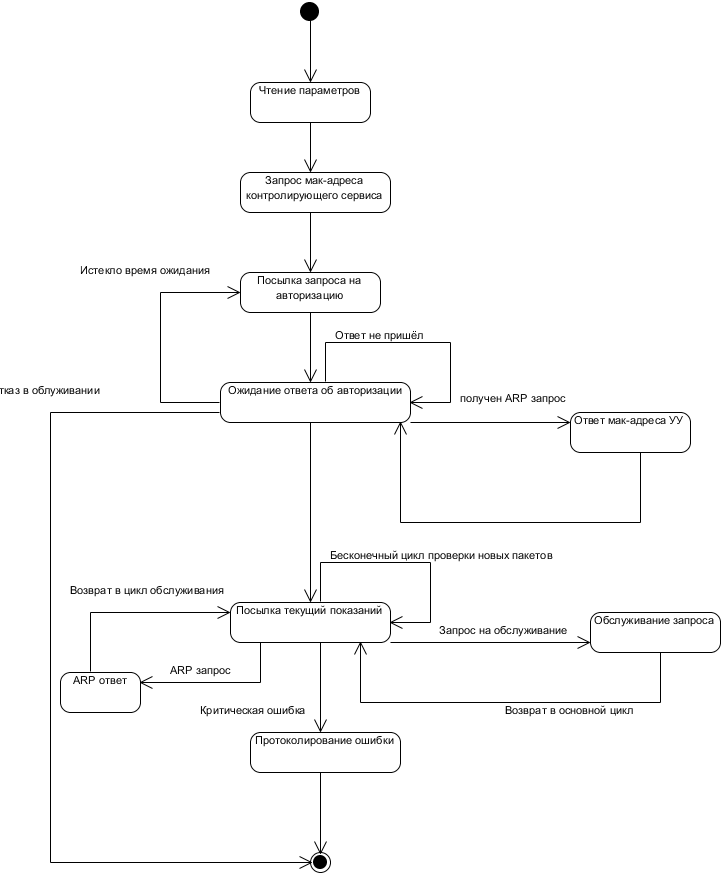
\includegraphics[bb=0 0 45 55, clip, scale=7.0]{dev_proto.png}}
	\caption{Протокол взаимодействия управляющего устройства и контролирующего сервиса}
	\label{img:devProto}
\end{figure}

Представленный конечный автомат реализует ARP ''How has'' запрос, ARP ''How has'' ответ --
минимально необходимое подмножество функций протокола ARP для работы в сетях Ethernet 802.3.
В качестве транспортного протокола передачи данных было принято решение использовать
протокол UDP, всвязи с ограниченным количеством оперативной памяти устройства управления, а так же
потому что алгоритм сетевого взаимодействия  предусматривает механизма повторения передачи
потерянных пакетов.


\subsubsection{Методика применения AES шифрования данных передаваемых
контролирующему сервису}
Одна из проблем решаемых в процессе разработки сетевого протокола 
взаимодействия управляющего устройства и контролирующего сервиса
была проблема обеспечения безопасности передаваемых данных.


Контролирующий сервис определяет, что принятые данные действительны
сравнивая пароль указанный в заголовке сетевого пакета. Однако,
при использования такого подхода, злоумышленник может прослушав
проходящий сетевой трафик получит этот пароль и использовать его
для формирования ложных запросов.


Для того, что бы избежать этого, заголовок пакета, содержащий пароль
и набор аппаратно-специфичных данных, должен подвергаться дополнительному
кодированию с использованием секретного ключа, известного только
авторизованному устройству и контролирующему сервису.


В качестве алгоритма кодирования данных заголовка пакета был использован
Advanced Encryption Standard. AES -- симметричный алгоритм блочного
шифрования, принятый в качестве стандарта шифрования правительством США
по результатам конкурса, организованного NIST в 1997 году, для замещения
алгоритма DES.


Причиной выбора именно этого алгоритма кодирования является
наличие аппаратной поддержки AES в микроконтроллерах XMega.


Благодаря наличию этого аппаратного модуля, процедура кодирования
по алгоритму AES со стороны программного обеспечения микроконтроллера
сводиться к следующим шагам:
\begin{enumerate}
    \item{} загрузить данные ключа в область памяти $AES.KEY$
        переферийного устройства AES кодирования;
    \item{} загрузить шифруемые данные в область памяти $AES.STATE$;
    \item{} установить параметры шифрования и флаг $AES\_START\_bm$ начала
        процедуры шифрования в конфигурационном регистре $AES.CTRL$;
    \item{} дождаться завершения шифрования, о чём сигнализирует
        флаги состояния в регистре состояния $AES.STATUS$;
    \item{} в зависимости от значения статуса, либо считать зашифрованные
        данные из области памяти $AES.STATE$, либо сообщить об ошибке
        шифрования.
\end{enumerate}
